\documentclass[10pt,a4paper]{article}
\usepackage{amsmath}
\usepackage[T1]{fontenc}
\usepackage[utf8]{inputenc}
\usepackage{lmodern,microtype,graphicx,tabularx,booktabs,array,enumitem,caption,fancyhdr,titlesec,hyperref,eurosym}
\usepackage[table]{xcolor}
\usepackage[left=19mm,right=19mm,top=23mm,bottom=18mm,headheight=15pt,headsep=7mm,footskip=10mm]{geometry}
\definecolor{ink}{HTML}{18364A}
\definecolor{accent}{HTML}{087E74}
\definecolor{muted}{HTML}{536573}
\definecolor{tablehead}{HTML}{EEF2F4}
\definecolor{tablerule}{HTML}{DDE4E8}
\definecolor{tablefinal}{HTML}{EDF7F3}
\hypersetup{colorlinks=true,urlcolor=accent,linkcolor=ink,pdftitle={Beyond the hourly average: AET challenge},pdfauthor={Team ApplePi}}
\titleformat{\section}{\large\sffamily\bfseries\color{ink}}{}{0pt}{}
\titlespacing*{\section}{0pt}{10pt}{5pt}
\setlength{\parindent}{0pt}
\setlength{\parskip}{5pt}
\setlist[itemize]{leftmargin=13pt,topsep=3pt,itemsep=2pt,parsep=0pt}
\captionsetup{font=small,labelfont=bf,skip=5pt,justification=raggedright,singlelinecheck=false}
\pagestyle{fancy}\fancyhf{}
\fancyhead[L]{\small\sffamily\bfseries\color{ink}NEURAL WAVE 2026\enspace /\enspace AI HACKATHON}
\fancyhead[R]{\small\sffamily\color{muted}AET challenge}
\fancyfoot[L]{\small\sffamily\color{muted}TEAM APPLEPI}
\fancyfoot[R]{\small\sffamily\color{muted}\thepage\ /\ 3}
\renewcommand{\headrulewidth}{0.3pt}
\newcommand{\resulttable}{\setlength{\tabcolsep}{8pt}\renewcommand{\arraystretch}{1.26}\arrayrulecolor{tablerule}}
\begin{document}
\fontsize{10.5}{13}\selectfont
{\fontsize{23}{26}\selectfont\sffamily\bfseries\color{ink}Beyond the hourly average}\par
{\large\sffamily Quarter-hour electricity price reconstruction}\par
{\small\color{muted}Challenge proposed by \textbf{AET -- Azienda Elettrica Ticinese}}\par
\vspace{2pt}

\section{The challenge}
Our task was to reconstruct \textbf{96 quarter-hour electricity prices from 24 supplied hourly prices}, for each of four market zones. An hourly average hides movements between its four quarters. A more detailed curve could therefore help AET understand price differences within the hour and support valuation when electricity is delivered unevenly.

The challenge was to recover that detail without changing the hourly reference: the four reconstructed prices must average back to the supplied hourly price, within \textbf{0.0001 \euro{}/MWh}. We used the official price data and aimed for a solution we could both evaluate and explain.

\section{Approach: learn the shape, preserve the average}
Repeating each hourly price four times gives a flat baseline. Smooth interpolation improves on this, but misses sharper movements. Our EDA highlighted the importance of slope, leading us to a layered reconstruction.

The central idea is a baseline plus a learned shape correction:
\[
\widehat{P}_{h,q}
=\underbrace{B_{h,q}}_{\text{smooth baseline}}
+0.8\times\underbrace{R_{h,q}}_{\text{learned correction}}.
\]
For each hour $h$ and quarter $q$, we start from a smooth PCHIP baseline and add a learned correction combining slope, curvature and zigzag. The four corrections within each hour sum to zero, so its average stays unchanged. The fixed rules then adjust predictions while preserving that average.

\textbf{A learned correction.} Three LightGBM models, based on boosted decision trees, learn what the baseline misses: \textbf{slope} (rising or falling prices), \textbf{curvature} (middle versus outer quarters), and \textbf{zigzag} (alternating movements). These components change the within-hour shape without moving its average.

Inputs include the day's hourly curve, differences between zones, calendar information and earlier price patterns. The target day's actual quarter-hour prices are excluded. We train with absolute-error loss on the three component coefficients and select configurations using price-level MAE. The \textbf{80\% correction scale} improved development results; it is fixed, not confidence-based.

\textbf{Final adjustments.} Fixed rules align predicted shapes for zones with nearly equal hourly prices and restrict sign changes within an hour. All preserve the hourly mean. Together with increasing the boosting rounds from 500 to 1,000, they reduced development MAE by 1.5\%, improving all eight folds. These are empirical choices validated on this dataset, rather than market rules.


\section{Challenges and solutions}
\textbf{Missing information and fair validation.} Many quarter-hour profiles share the same hourly average, so some detail remains unpredictable. We used chronological validation and calendar-based history lookups to avoid future information and incorrect lags when dates are missing.

\textbf{Knowing when to stop adding complexity.} We explored Ridge, CatBoost, Random Forest, Extra Trees, temporal neural networks and graph models. Local-geometry features worsened the previous model's MAE from \textbf{3.9479 to 3.9497 \euro{}/MWh}. In a separate June--August comparison, a graph blend improved it from \textbf{4.2246 to 4.2058} (0.4\%). That gain was too small to justify the added complexity, so we retained LightGBM.

\newpage
\section{Results: more detail, less reconstruction error}
We measure accuracy with mean absolute error (MAE): the average distance between reconstructed and observed prices. Each evaluation day and zone has equal weight; lower is better. The final model reduces MAE by \textbf{52.2\% on development dates} and \textbf{54.1\% on September}, compared with repeating hourly prices.

Development uses eight chronological January--August folds, training on earlier dates and scoring days 19 through month-end. September covers 19--30 September, with training through August. September was examined in several experiments before the final changes, so it is a \textbf{historical assessment, not an untouched final test}.

\begin{center}
\resulttable
\begin{tabularx}{\linewidth}{*{3}{>{\raggedright\arraybackslash}X}}
\rowcolor{tablehead}\textbf{Method} & \textbf{Development MAE} & \textbf{September MAE}\\\hline
Flat hourly prices & 8.13 & 10.90\\\hline
PCHIP baseline & 5.62 & 6.93\\\hline
Full correction (scale 1.0) & 3.98 & 5.43\\\hline
Previous model (no rules) & 3.95 & 5.04\\\hline
\rowcolor{tablefinal}\textbf{Final model} & \textbf{3.89} & \textbf{5.00}\\\hline
\end{tabularx}
\captionof{table}{Average price error in \euro{}/MWh. All September scores use the same dates. The previous model uses 500 boosting rounds and no final adjustment rules; the final model uses 1,000 rounds and the rules.}
\end{center}

\begin{center}
\resulttable
\begin{tabularx}{\linewidth}{*{4}{>{\raggedright\arraybackslash}X}}
\rowcolor{tablehead}\textbf{Zone} & \textbf{Model MAE} & \textbf{Flat MAE} & \textbf{Error reduction}\\\hline
ZONE\_0 & 3.83 & 10.78 & \textcolor{accent}{64.5\%}\\\hline
ZONE\_1 & 6.12 & 13.30 & \textcolor{accent}{54.0\%}\\\hline
ZONE\_2 & 5.49 & 9.72 & \textcolor{accent}{43.5\%}\\\hline
ZONE\_3 & 4.57 & 9.79 & \textcolor{accent}{53.3\%}\\\hline
\end{tabularx}
\captionof{table}{September results by zone. Reductions compare the final model with flat hourly prices and are calculated before rounding. Source: \texttt{results/summary.csv}.}
\end{center}

The model improves on flat prices in every zone. The final changes bring a smaller September gain over the previous model (0.8\%), with ZONE\_3 slightly worse (4.57 versus 4.55). These are price-accuracy results; effects on trading or portfolio valuations have not been measured.

\begin{center}
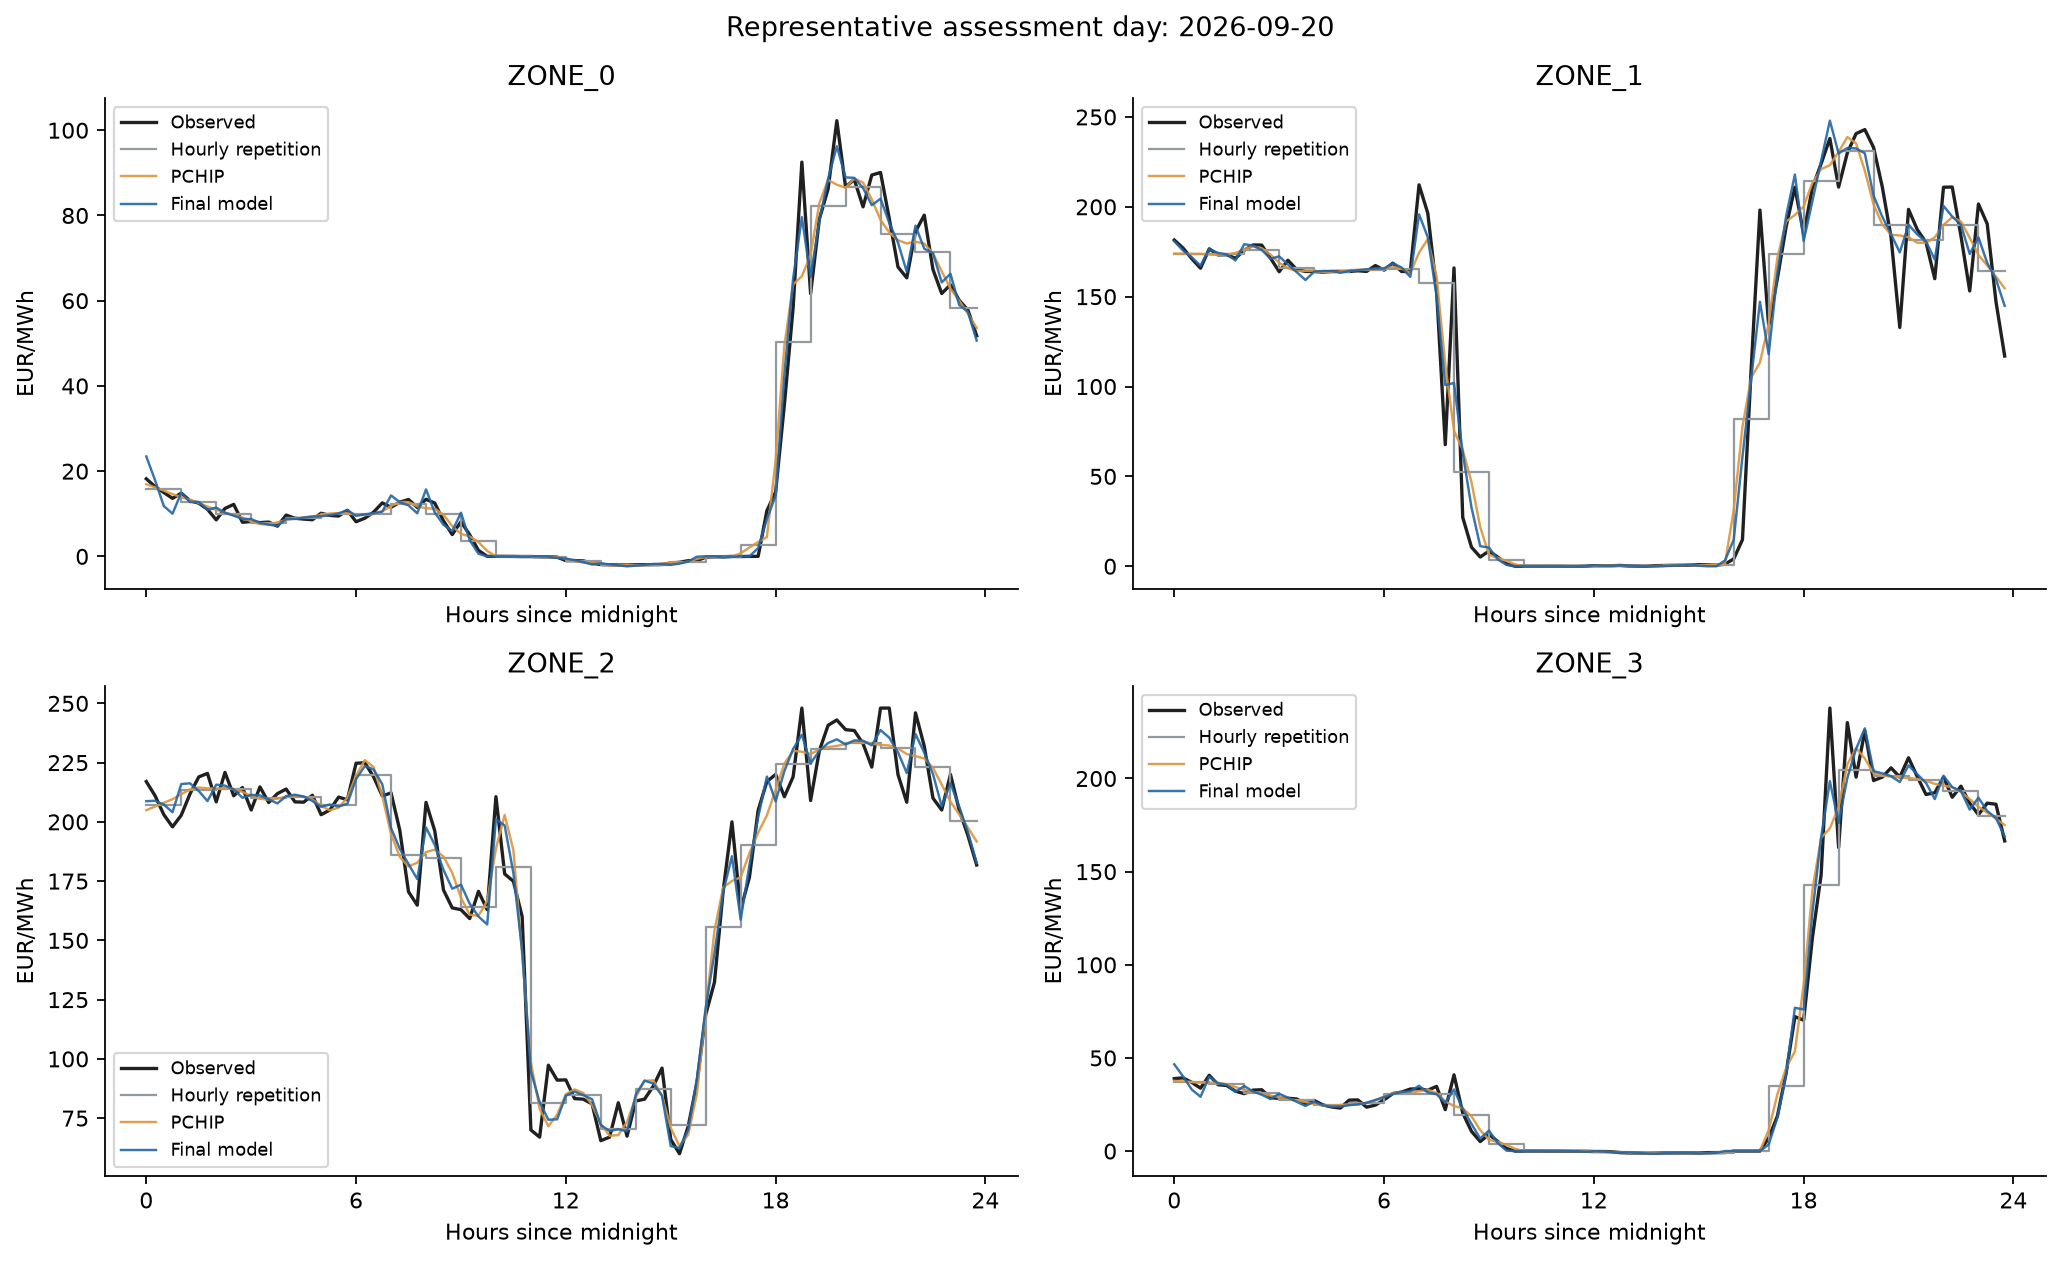
\includegraphics[width=0.76\linewidth]{images/representative_reconstruction.png}
\captionof{figure}{Reconstruction on 20 September 2026 across all four zones. The observed curve shows both where the model recovers detail and where sharp movements remain difficult.}
\end{center}



\newpage
\section{Dashboard: making the predictions understandable}
We also wanted someone without a machine-learning background to be able to explore the results. The dashboard brings together \textbf{Model Results}, \textbf{Understanding the Model}, \textbf{Risk Alerts} and the \textbf{Data Story}. Users can compare price curves, inspect one hour's component contributions and see the signal behind its risk flag.

\begin{center}
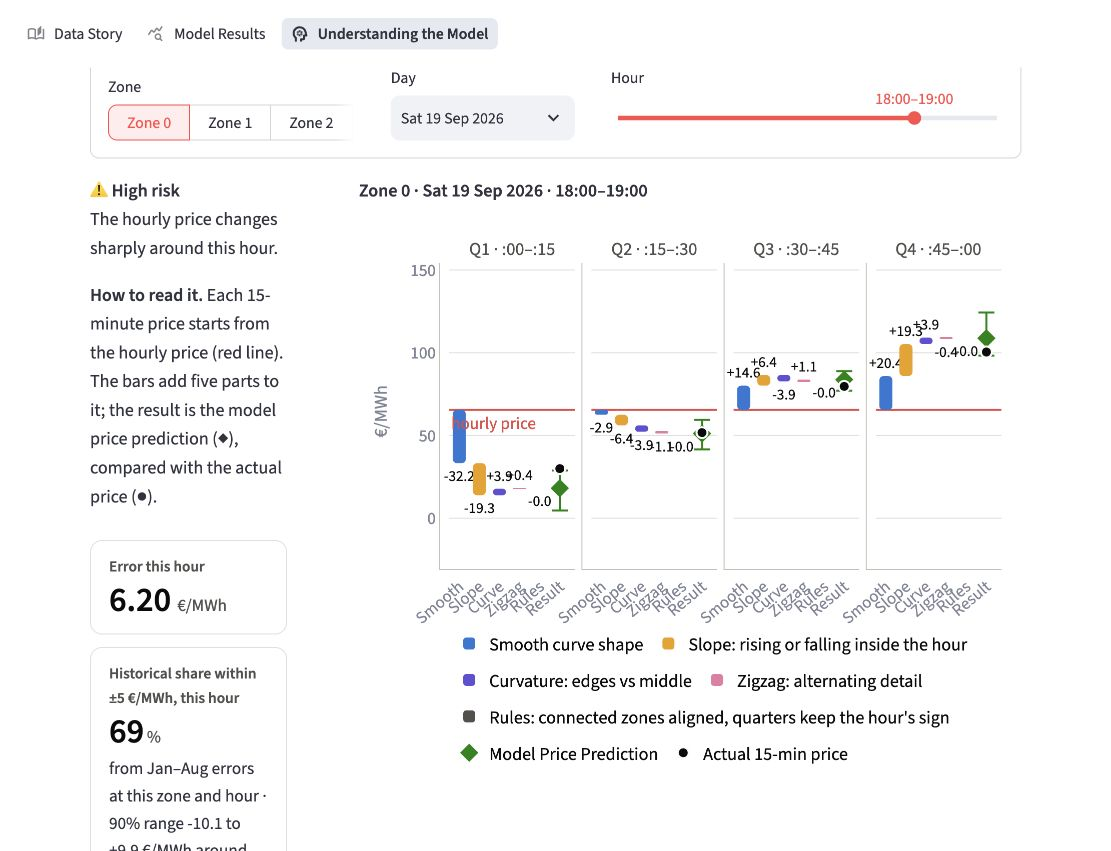
\includegraphics[width=0.82\linewidth,trim=0 76bp 0 55bp,clip]{images/dashboard_detail.png}
\captionof{figure}{ZONE\_0, 19 September 2026, 18:00--19:00. The dashboard separates the smooth curve, learned corrections and fixed rules, and compares the result with observed prices.}
\end{center}

\section{Does the risk indicator identify harder hours?}
The indicator combines hourly ramps, daily variability and recent historical reconstruction difficulty. On development folds, high-risk hours had \textbf{2.8--3.9 times the MAE} of low-risk hours. This suggests that the labels identify harder conditions, but they are \textbf{heuristics, not calibrated confidence probabilities} or guarantees for individual predictions.

\begin{center}
\resulttable
\begin{tabularx}{\linewidth}{*{4}{>{\raggedright\arraybackslash}X}}
\rowcolor{tablehead}\textbf{Zone} & \textbf{Low-risk MAE} & \textbf{High-risk MAE} & \textbf{High / low}\\\hline
ZONE\_0 & 1.51 & 5.89 & 3.9$\times$\\\hline
ZONE\_1 & 2.80 & 8.32 & 3.0$\times$\\\hline
ZONE\_2 & 2.03 & 5.68 & 2.8$\times$\\\hline
ZONE\_3 & 2.22 & 7.20 & 3.2$\times$\\\hline
\end{tabularx}
\captionof{table}{Observed group MAE in \euro{}/MWh on January--August development folds. These reused folds provide development evidence, not an independent final test of the indicator.}
\end{center}

\section{AI agents and LLM usage}
We worked with LLM-based coding assistants throughout the project, especially when coding. It was an iterative process: we tried an approach, looked at the results, and used the assistants to help identify errors and work through possible solutions. We also discussed our EDA findings with them to explore features and model changes worth testing. We checked suggestions through tests and backtesting, keeping changes supported by the results. Finally, we used them to help organise and revise the repository, report and presentation through several rounds of feedback.

{\small The papers, libraries and challenge materials we consulted are listed in \texttt{docs/REFERENCES.md} in the repository, including approaches tested but not retained.}
\end{document}
